%%%%%%%%%%%%%%%%%%%%%%%%%%%%%%%%%%%%%%%%%%%%%%%%%%%%%%%%%%%%%%%%%%%%%%%%%%%%%%%%
%%
%%   BornAgain User Manual
%%
%%   homepage:   http://www.bornagainproject.org
%%
%%   copyright:  Forschungszentrum Jülich GmbH 2015
%%
%%   license:    Creative Commons CC-BY-SA
%%   
%%   authors:    Scientific Computing Group at MLZ Garching
%%               C. Durniak, M. Ganeva, G. Pospelov, W. Van Herck, J. Wuttke
%%
%%%%%%%%%%%%%%%%%%%%%%%%%%%%%%%%%%%%%%%%%%%%%%%%%%%%%%%%%%%%%%%%%%%%%%%%%%%%%%%%


\newpage
\chapter{Software architecture}\SecLabel{SoftwareArchitecture}
 

%%%%%%%%%%%%%%%%%%%%%%%%%%%%%%%%%%%%%%%%%%%%%%%%%%%%%%%%%%%%%%%%%%%%%%%%%%%%%%%%
\section{Basic structure of \BornAgain}
%%%%%%%%%%%%%%%%%%%%%%%%%%%%%%%%%%%%%%%%%%%%%%%%%%%%%%%%%%%%%%%%%%%%%%%%%%%%%%%%

\BornAgain\ is written in \Code{C++}
and uses an object oriented approach to 
achieve modularity, extensibility and transparency.
This leads to the task driven rather than the command driven approach in 
different aspects of the simulation and fitting of GISAS data.
The user defines the sample structure, beam and detector characteristics and
fit parameters using building
blocks -- \Code{classes} -- defined in core libraries of the framework.
These buildings blocks are combined by the user according to his current
task using one the following approaches:
\begin{itemize}
\item The user creates a \Python\ script with a sample description and simulation settings
using the \BornAgain\ API.
The user then runs the simulation by executing the script in the \Python\ interpreter and assesses the
simulation results using his preferred graphics or analysis library, e.g. \Python\ + \Code{numpy} + \Code{matplotlib}.
\item The user may write a standalone \Code{C++} application linked to the \BornAgain\ libraries.
\item The user interacts with the framework through a graphical 
user interface (forthcoming).
\end{itemize}

The object oriented approach in the software design allows users 
to have a much higher level of flexibility in the sample construction; it also
decouples the building blocks used in the internal calculations and thereby facilitates the creation of new models,
with little or no modification to the existing code. 


\begin{figure}[htbp]
\centering
  \resizebox{0.9\textwidth}{!}{%
    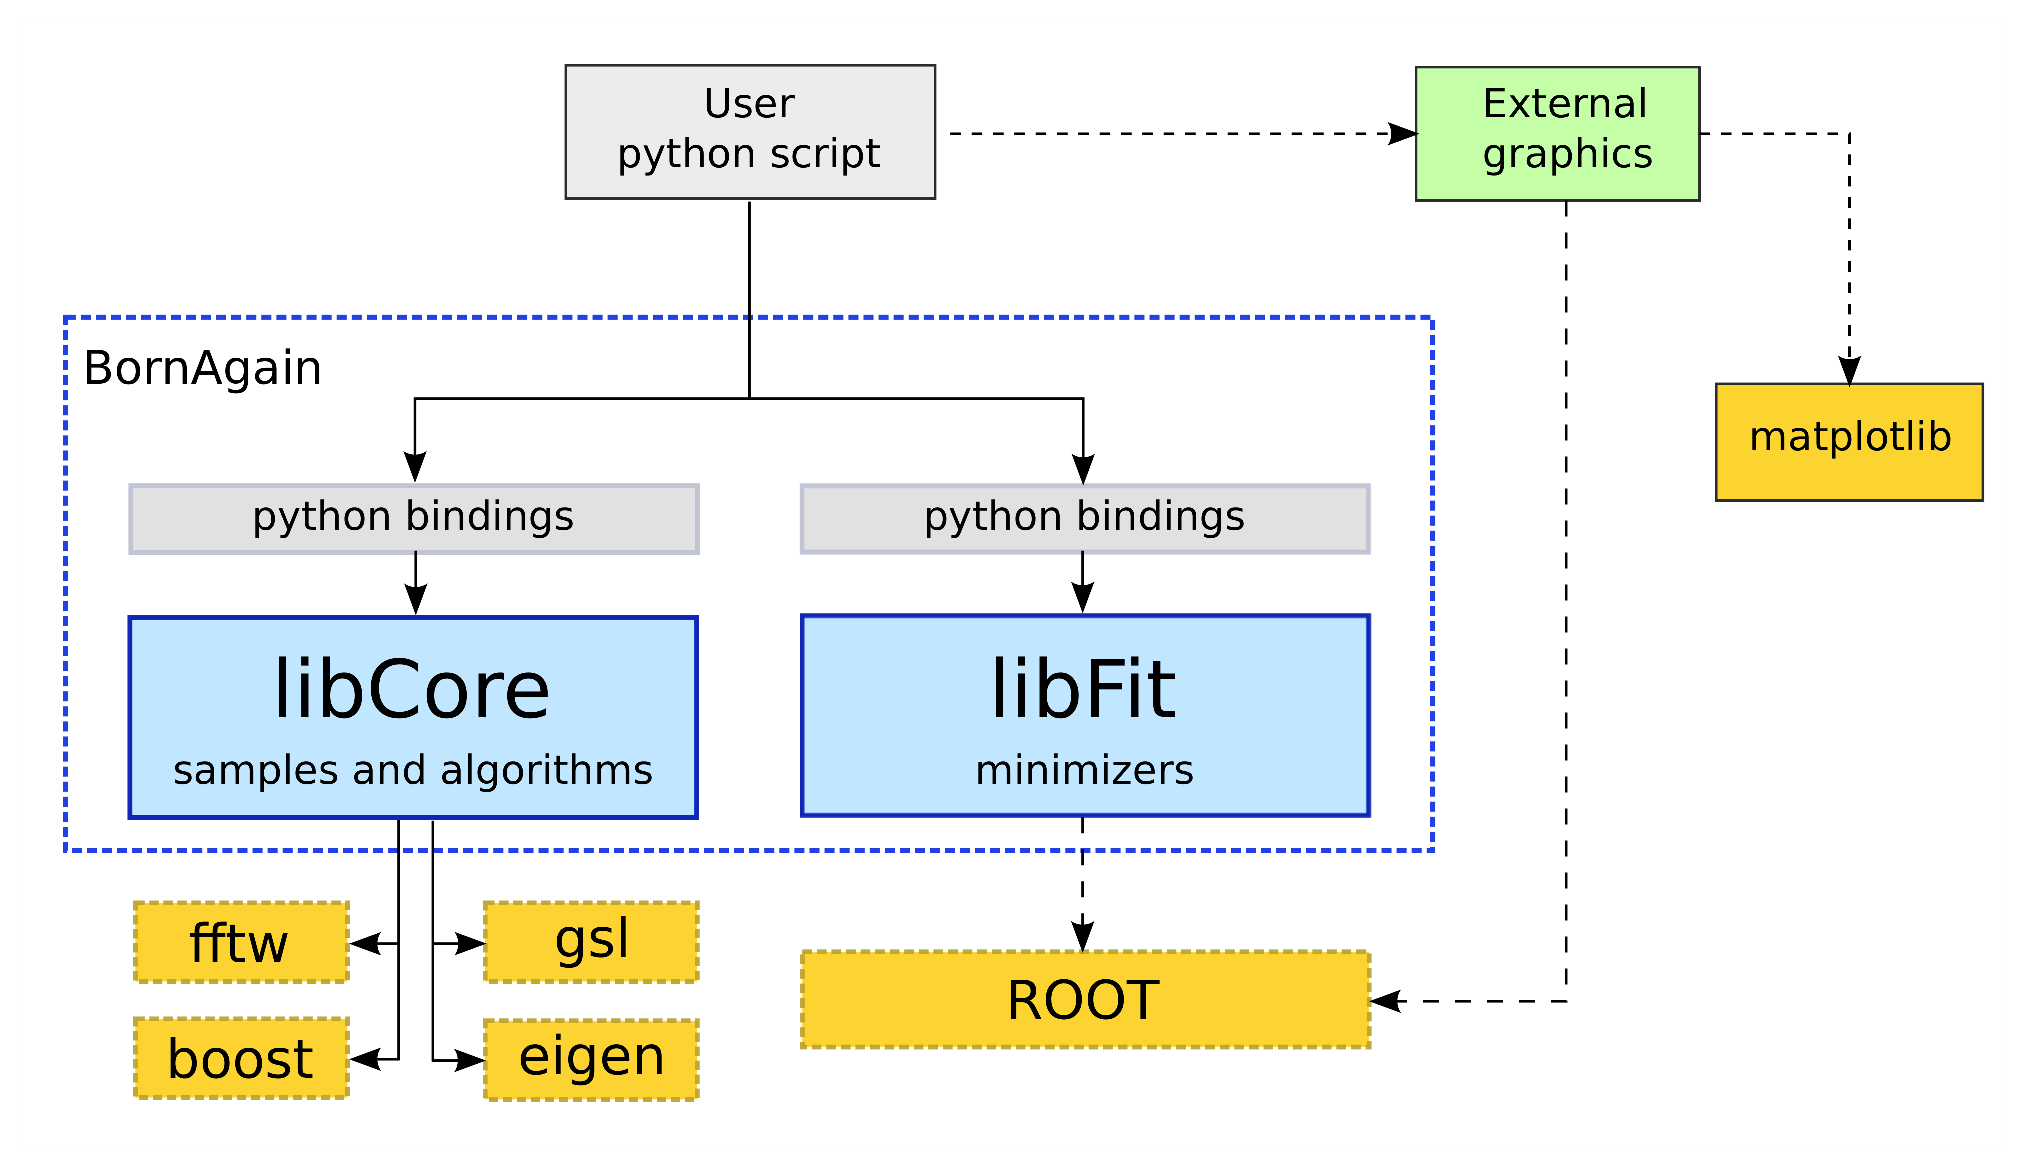
\includegraphics{fig/drawing/basic_architecture.eps}}
\caption{Structure of \BornAgain\ libraries.}
\label{fig:two_ratios}
\end{figure}


The general structure of \BornAgain\ and the way the user interacts with it are
shown in Fig.~\ref{fig:two_ratios}.
The framework consists of two shared libraries, \Code{libBornAgainCore} and
\Code{libBornAgainFit}. Thanks to the \Python\ interface they can be imported into \Python\ as external modules. The library \Code{libBornAgainCore} contains a number of classes, grouped into several class categories, necessary for the description of a model and running a simulation.
The library  \Code{libBornAgainFit} contains a number of minimization engines 
and interfaces to them, allowing the user to fit real data with the model previously defined.

\BornAgain\ depends on a few external and well established
open-source libraries: \Code{boost}, GNU scientific library, Eigen and
Fast Fourier Transformation libraries. They are required to be
installed on the system to run \BornAgain\ on Unix Platforms. In the
case of Windows Platform they are added to the system automatically during \BornAgain\ installation. Other libraries shown
on the plot (\Code{ROOT}, \Code{matplotlib}) are optional.

 
%%%%%%%%%%%%%%%%%%%%%%%%%%%%%%%%%%%%%%%%%%%%%%%%%%%%%%%%%%%%%%%%%%%%%%%%%%%%%%%%
\section{Data classes for simulations and fits}
%%%%%%%%%%%%%%%%%%%%%%%%%%%%%%%%%%%%%%%%%%%%%%%%%%%%%%%%%%%%%%%%%%%%%%%%%%%%%%%%

This section will give an overview of the classes that are used to describe all the data needed to perform a single simulation. The prime elements of this data are formed by the sample, the experimental conditions (beam and detector parameters) and simulation parameters.

These classes constitute the main interface to the software's users, since they will mostly be interacting with the program by creating samples and running simulations with specific parameters. Since it is not the intent to explain internals of classes in this document, the text and figures will only mention the most important methods and fields of the classes discussed. Furthermore, getters and setters of private member fields will not be indicated, although these do belong to the public interface. For more detailed information about the project's classes, their methods and fields, the reader is referred to the source code documentation. REF?



\subsection{The Experiment object}
The \Code{Experiment} class holds all references to data objects that are needed to perform a simulation. These consist in a sample description, possibly implemented by a builder object, detector and beam parameters and finally, a simulation parameter class that defines the different approximations that can be used during a simulation. Besides getters and setters for these fields, the class also contains a \Code{runSimulation()} method that will generate an ISimulation object that will perform the actual computations. The class diagram for \Code{Experiment} is shown in \reffig{exp}.

\vspace{8mm}
\begin{figure}[H]
%the makebox macro ensures centering of the resulting figure
\makebox[\textwidth][c]{
\begin{tikzpicture}
\begin{umlpackage}{Simulation Data}
\umlclass{Experiment}{
  -- mp\_sample : ISample* \\
  -- mp\_sample\_builder : ISampleBuilder* \\
  -- m\_detector : Detector \\
  -- m\_beam : Beam \\
  -- m\_intensity\_map : OutputData<double> \\
  -- m\_sim\_params : SimulationParameters
}{
  \umlvirt{+ clone() : Experiment*} \\
  \umlvirt{+ runSimulation() : void} \\
  \umlvirt{+ normalize() : void}
}
\umlemptyclass[x=7, y=0]{ISample}
\umlemptyclass[x=7, y=-2]{Detector}
\umlemptyclass[x=7, y=-4]{Beam}
\umlemptyclass[x=7, y=-6]{SimulationParameters}
\umlemptyclass[y=-4]{GISASExperiment}
\umluniassoc[geometry=|-, anchor1=0]{Experiment}{ISample}
\umluniassoc[geometry=|-, anchor1=0]{Experiment}{Detector}
\umluniassoc[geometry=|-, anchor1=0]{Experiment}{Beam}
\umluniassoc[geometry=|-, anchor1=0]{Experiment}{SimulationParameters}
\umlinherit[geometry=--]{GISASExperiment}{Experiment}

\umlnote[y=-6.5, width=6cm]{GISASExperiment}{
  The ``runSimulation()'' method retrieves an ISimulation object
  from the topmost ISample object and calls its ``run()'' method 
  to perform the actual computations.
}
\end{umlpackage}
\end{tikzpicture}
} %end makebox
\caption{The Experiment class as a container for sample, beam, detector and simulation parameters.}
\label{fig:exp}
\end{figure}

\subsection{The ISample class hierarchy}

Samples are described by a hierarchical tree of objects which all adhere to the ISample interface. The composite pattern is used to achieve a common interface for all objects in the sample tree. The sample description is maximally decoupled from all computational classes, with the exception of the ``createDWBASimulation()'' method. This method will create a new object of type ``DWBASimulation'' that is capable of calculating the scattering contributions originating from the sample part in question. This coupling is not very tight however, since the ISample subclasses only need to know about which class to instantiate and return.

This interface and two of its subclasses are sketched in \reffig{isample}.

\vspace{8mm}

\begin{figure}[H]
\makebox[\textwidth][c]{
\begin{tikzpicture}
\begin{umlpackage}{Sample description} 
% Code from official documentation goes here...
\umlinterface{ISample}{
}{
  \umlvirt{+ clone() : ISample*} \\
  \umlvirt{+ createDWBASimulation() : DWBASimulation*}
}
\umlclass[y=-4]{MultiLayer}{
  -- m\_layers : std::vector<Layer *> \\
  -- m\_interfaces : std::vector<LayerInterface *>
}{
  + getNumberOfLayers() : size\_t \\
  + getNumberOfInterfaces() : size\_t \\
  + addLayer(const Layer \&layer) : void
}
\umlclass[x=8,y=-4]{Layer}{
  -- mp\_material : IMaterial* \\
  -- m\_thickness : double
}{
  + getThickness() : double \\
  + setThickness(double thickness) : void
}
\umlinherit[geometry=-|]{MultiLayer}{ISample}
\umlinherit[geometry=|-]{Layer}{ISample}
\umluniassoc[geometry=--, mult2=n]{MultiLayer}{Layer}
\end{umlpackage}
\end{tikzpicture}
}
\caption{The ISample interface}
\label{fig:isample}
\end{figure}



\subsection{The FitSuite class} \SecLabel{FitSuiteClass}

\subsection{The IMinimizer class} \SecLabel{IMinimizerClass}

\subsection{The MinimizerOptions class} \SecLabel{MinimizerOptionsClass}
